\chapter{对偶理论}\label{chap:duality}

在经济社会中,通常会有买家和卖家两种角色. 卖家要以尽可能高的售价卖出商品,而买家则希望以尽可能低的价格购买商品. 因此,卖家和买家之间构成了相互矛盾的利益关系. 下面我们来看一个具体的例子. 

甲用三种纸浆混合生产两种抽纸. 甲的目标是让总售价最大. \Cref{tab:cleaner-intro} 描述了公司甲用纸浆生产抽纸的信息表. 
\begin{table}[ht]
        \centering
        \begin{tabular}{c|ccc|c}
        \hline
            & 纸浆1&纸浆2&纸浆3&售价(万元/吨) \\
            \hline
             抽纸A  & 0.25&0.50&0.25&12 \\
             抽纸B  & 0.50&0.50& &15\\
             \hline
             库存(吨)&120&150&50& \\
             \hline
        \end{tabular}
        \caption{抽纸和纸浆信息表,其中,数据的第一(二)行表示生产一吨抽纸A(B)需要的纸浆吨数. }
        \label{tab:cleaner-intro}
\end{table}

设抽纸A和B分别生产$x_1$和$x_2$吨,我们可以把甲的目标写成一个优化问题:
\begin{align*}
\begin{array}{rrcl}
\displaystyle\maximize_{x_1,x_2}\quad&\multicolumn{3}{l}{z=12x_1+15x_2}\\
\text{s.t.}\quad&0.25x_1+0.50x_2&\le&120,\\
&0.50x_1+0.50x_2&\le&150,\\
&0.25x_1&\le& 50,\\
&x_1&\ge& 0,\\
&x_2&\ge& 0.
\end{array}
\end{align*}

当然,甲也有一种选择,自己不生产销售纸巾,而是直接售卖纸浆. 此时,甲变成了卖家. 现在有一个公司乙需要这三种纸浆,打算向甲购买,问甲应该如何定价纸浆?

假设三种纸浆的定价分别为每吨$y_1,y_2,y_3$万元. 对于买家乙来说,它希望总价格尽量小,但不能低于甲用纸浆生产抽纸所产生的价值,因此,对于乙来说,优化问题为:
\[
 \begin{array}{rrcl}
\displaystyle\minimize_{y_1,y_2,y_3}\quad&\multicolumn{3}{l}{w=120y_1+150y_2+50y_3} \\
\text{s.t.}\quad& 0.25y_1+0.50y_2+0.25y_3&\ge&12,\\
&0.50y_1+0.50y_2&\ge&15,\\
&y_1&\ge&0,\\
&y_2&\ge&0,\\
&y_3&\ge&0.
 \end{array}
\]

假设甲乙双方都知道\Cref{tab:cleaner-intro} 的信息,如果甲对纸浆的定价高于上述乙优化问题的最优解,那么乙会选择不购买纸浆. 此时,这一市场的资源配置发生了浪费:甲有多余的纸浆,乙没有得到所需的纸浆.

在上个世纪,苏联完全实行计划经济,一个东西的售价是多少,由国家计划决定,而不是由市场决定. 我们上面的小例子就是计划经济的一个缩影:如果没有合理的定价,社会资源的配置就会出现问题,想买的买不到,想卖的卖不出去.

1959年,苏联经济学家Kantorovich出版了著作《经济资源的最佳利用》,第一次将上面线性规划的这种思路引入到资源配置中. 对于一个资源配置高效的经济社会,每一个产品的定价都应该接近于它对应优化问题的最优解,这样的定价被称为\textit{影子价格}. 

1965年,因Kantorovich因为这一工作而获列宁奖金. 1975年,Kantorovich因此获得了诺贝尔经济学奖,成为第一个获得这一奖项的前苏联经济学家. 

在我们上面纸浆定价的例子中,我们其实看到了两个优化问题之间非同寻常的联系:一个的目标函数是另一个的约束条件. 影子价格产生于两个最优解相等的情况,正是Kantorovich所观察到的核心现象. 

这样的现象被称为\textit{对偶性},对偶性不仅仅是线性规划中的现象,它是优化问题中的一个普遍现象. 在本章中,我们考虑带约束的优化问题. 它的一般形式是
\begin{equation}
\begin{aligned}
    \minimize_x\quad& f(x) \\
    \text{s.t.}\quad& h(x)=0,\\
    & g(x)\leq 0, \\
    & x \in \Omega.
\end{aligned}\label{eq:general-constraint}    
\end{equation}
函数$f:\R^n\to \R$是目标函数,$h:\R^n\to \R^m$和$g:\R^n\to \R^p$分别是等式约束和不等式约束. 我们假设$
,h,g$都是连续的,且通常假设它们拥有连续的二阶导数.

一个满足所有函数约束的点$x\in\Omega$被称作\textbf{可行解},而使得$f$取得最小值的可行解叫做\textbf{最优解}. 有时候优化问题的目标可能是最大化$f$,此时相应的最优解就是使得$f$取得最大值的可行解. 本章的任务是讨论各种情况下最优值的必要条件,这些必要条件最终推导出了\textbf{对偶理论}. 

\section{约束的几何意义}\label{sec:constraint-geometry}

我们首先指出,优化问题的函数约束其实有很强的几何意义,更偏微积分的讨论请参见\Cref{chap:calculus}. 我们先只关注 \eqref{eq:general-constraint} 中的等式约束$h(x)=0$,考虑如下例子. 

\begin{example}[二维空间中的约束]\label{ex:2d-constraint}
考虑二维空间中的如下约束:
\begin{align*}
    h_1(x)&=x_1^2+x_2^2-1=0,\\
    h_2(x)&=x_1+x_2-1=0.
\end{align*}
第一个约束$h_1(x)=0$定义了一个圆环,它是一维曲面\footnote{严格来说,一维空间应该叫曲线. 不过,为了和后面高维空间的术语保持一致,我们都称之为曲面. }. 第二个约束$h_2(x)=0$定义了一条直线,也是一维曲面. 这两个约束的交集是两个点,即零维曲面.
\end{example}

\begin{example}[三维空间中的约束]\label{ex:3d-constraint}
考虑三维空间中的如下约束:
\begin{align*}
    h_1(x)&=x_1^2+x_2^2+x_3^2-1=0,\\
    h_2(x)&=x_1+x_2+x_3-1=0.
\end{align*}
第一个约束$h_1(x)=0$定义了一个球面,它是一个二维曲面. 第二个约束$h_2(x)=0$定义了一个平面,也是一个二维曲面. 这两个约束的交集是一个圆环,即一维曲面.
\end{example}

我们可以从另一个角度来理解这两个例子. 在\Cref{ex:2d-constraint} 中,原本$(x_1,x_2)$两个维度都是自由选择的,所以我们可以用两个互相独立的参数来描述这个点. 当加入约束$h_1(x)=0$之后,给定一个$x_1$,我们我们并不能自由选择$x_2$,而是要满足约束$h_1(x)=0$. 容易看出,我们只用一个参数$\theta$就可以描述这个约束下的点:
\[
(x_1,x_2)=(\cos\theta,\sin\theta),\quad \theta\in[0,2\pi).
\]
所以,约束$h_1(x)=0$将原本的二维空间约束到了一维空间. 继续加入约束$h_2(x)=0$,我们已经不需要参数就可以描述这个约束下的点:
\[
(x_1,x_2)\in\{(0,1),(1,0)\}.
\]
因此,约束$h_2(x)=0$将原本的一维空间约束到了零维空间.

类似地,在\Cref{ex:3d-constraint} 中,原本$(x_1,x_2,x_3)$可以用三个互相独立的参数来描述,当加入约束$h_1(x)=0$之后,我们只能用两个独立的参数来描述,而加入约束$h_2(x)=0$之后,我们只需要一个参数就可以描述这个约束下的点. 这对应的就是三维空间被约束到了二维空间,再被约束到了一维空间.

更一般地,如果$h:\R^n\to\R^m$,那么$h$的每一维都对$\R^n$增加了一个约束,最终$h(x)=0$定义了一个$n-m$维的曲面(在通常的情况下). 

不过,这一性质并不是绝对的,请看下面的例子. 

\begin{example}\label{ex:3d-constraint-2}
在三维空间中,考虑如下约束:
\begin{align*}
    h_1(x)&=x_1^2+x_2^2+x_3^2-1=0,\\
    h_2(x)&=x_1=1.
\end{align*}
容易看出,这一约束其实对应的是一个点$(1,0,0)$,即零维曲面,而不是我们预期的一维曲面.

再考虑如下约束:
\begin{align*}
    h_1(x)&=x_1+x_2+x_3=1,\\
    h_2(x)&=x_1+2x_2+3x_3=1,\\
    h_3(x)&=x_2+2x_3=0.
\end{align*}
这一约束对应的是一个直线,即一维曲面,而不是我们预期的零维曲面.
\end{example}

上面的例子是很恼人的,因为我们无法通过直观的方式来判断曲面的维度. 所以,我们需要一些更强的方法来判断曲面的维度. 如果$h$是具有连续的一阶导数的函数,那么这个曲面是\textit{光滑}\footnote{在文献中,“光滑”这一词的含义有多种多样,例如无穷次可微、具有连续二阶导数等等. 因此,这里用光滑仅仅只是方便起见,在阅读文献时,需要根据具体的上下文来理解这一词的含义.}的. 我们只考虑光滑曲面,因为它们是最常见的情况.

\Cref{ex:3d-constraint-2} 的第一个约束为什么不符合预期?在点$(1,0,0)$,球面$h_1(x)=0$的切平面恰好是$x_1=1$,这意味着在这个点,$h_1(x)=0$和$h_2(x)=0$其实只产生了一个有效的约束!这说明,“切平面”这样的概念对于维度有着至关重要的作用. 
    
在一般空间中,我们可以通过\textit{切空间}的概念来描述曲面在某个点的维度. 切空间其实是所有过该点的切线的集合. 为了引入切线,我们先介绍曲线,
\begin{definition}[曲线和切向量]
    考虑曲面$S$,其上的一条\textbf{曲线}是一系列点的集合:$x(t)\in S$,它们以$t\in[0,1]$为参数且在该区间上连续. 因为它只有一个参数,所以它是一维曲面. 

    如果曲线$x(t)$在点$x^*=x(t^*)$处可微,那么它在该点的\textbf{导数}被定义为
    \[\dot{x}(t)=\left.\frac{\d x(t)}{\d t}\right|_{t=t^*}.\]
    如果曲线处处可微,我们称它是\textbf{可微的}. 

    考虑向量$v$,如果存在一个可微曲线$x(t)$和常数$k>0$,使得
    \[\dot{x}(0)=kv,\quad x(0)=x^*,\]
    那么我们称$v$是曲面$S$在点$x^*$处的\textbf{切向量}.
\end{definition}

有了曲线和切向量的概念,我们可以引入切空间的概念. 

\begin{definition}[切空间]
    考虑曲面$S$,在点$x^*\in S$处的\textbf{切空间}是所有在该点的切向量的集合,记作$T_{x^*}(S)$.
\end{definition}

下面我们看一个切空间的例子.

\begin{example}[三维球面的切空间]\label{ex:tan-space}
    考虑三维空间中的单位球面
    \[S^2=\{x\in\R^3:x_1^2+x_2^2+x_3^2=1\}.\]
    在点$x^*=(1,0,0)$处,球面的切空间是什么?我们可以通过曲线来描述切空间. 考虑过$x^*$的圆弧:
    \[x_\theta(t)=(\cos t,\sin t\cos\theta,\sin t\sin\theta), \quad t\in[0,\pi],\]
    其中$\theta$是一个固定的参数,它表示圆弧的方向. 那么,
    \[\dot{x}_\theta(0)=(0,-\sin\theta,\cos\theta),\]
    所以,$x^*$处的切空间至少包含以下集合
    \begin{align*}
        \{(0,-k\sin \theta,k\cos\theta):k\in\R,\theta\in[0,2\pi)\}= \{(0,y,z):y,z\in\R\}.
    \end{align*}
    因为球面是一个二维曲面,所以切空间不可能是整个三维空间. 因此,过$x^*$的切空间就是
    \[T_{x^*}(S^2)=\{(0,y,z):y,z\in\R\}.\]
\end{example}

\Cref{ex:tan-space} 中的切空间是一个二维的线性空间. 直观上,任何切空间都是应该一个线性空间,这也是它名字的来源. 
\begin{lemma}\label{lemma:tan-space}
    切空间是一个线性空间. 
\end{lemma}

尽管\Cref{lemma:tan-space} 的直观是很明显的,但是这一性质的证明需要一定程度的微积分知识,所以我们这里略去. 我们也只需要这一性质的直观理解,而不需要深入的数学推导.

既然切空间是一个线性空间,我们的一个主要目标就是给出切空间的显式表达. 这一部分需要一些基本的微积分和线性代数知识,请参阅\Cref{chap:calculus} 和\Cref{chap:linear-algebra}.

考虑一条曲线$x(t)$,如果它在$h_i(x)=0$形成的曲面上,所以
\[\forall t,h_i(x(t))=0\implies\forall t, \frac{\d}{\d t}h_i(x(t))=0.\]
那么,根据复合函数的求导法则,应该有
\[\frac{\d}{\d t}h_i(x(t))=0\iff \nabla_x h_i(x(t))\dot{x}(t)=0.\]
因此$x(t)$的切向量和该点处函数$h_i(x(t))$的导数向量正交. 

于是,如果$x(t)$在$h(x)=0$形成的曲面上,那么$x(t)$处的导数$\nabla h(x(t))$是切空间的法向量. 这一数学推导的示意图见\Cref{fig:tangent-space}.

\begin{figure}[ht]
\centering
    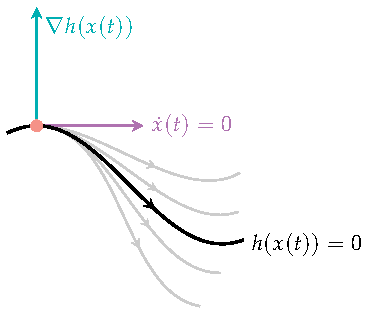
\includegraphics[width=0.6\textwidth]{figures/duality/tan-1dim.pdf}
\caption{切空间的法向量示意}
\label{fig:tangent-space}
\end{figure}

对于\Cref{ex:tan-space},我们可以看到,
\[\nabla h_1(x)=(2x_1,2x_2,2x_3)\implies \nabla h_1(x^*)=(2,0,0).\]
因此,切空间$T_{x^*}(S^2)$的法向量是$(2,0,0)$,我们可以重新描述切空间为一个二维平面
\[T_{x^*}(S^2): 2x_1+0x_2+0x_3=0\iff x_1=0.\]
这和\Cref{ex:tan-space} 的结果是一致的.

记
\[M=\left\{\sum_{i} \alpha_i \nabla h_i(x^*)^\t:\alpha_i\in\R\right\},\]
即$M$是$\nabla h_i(x^*)^\t$张成的空间. 它的正交补是
\[M^\perp=\{{y}\in\R^n:\nabla {h(x^*)y}=0\},\]
这里,$\nabla {h(x^*)}$是$h$在$x^*$处的Jacobi矩阵,即对$h$的每一个分量求导得到的矩阵:
\[\nabla {h(x^*)}=\begin{pmatrix}
    \nabla h_1(x^*)\\
    \nabla h_2(x^*)\\
    \dots\\
    \nabla h_m(x^*)
\end{pmatrix}.\]

我们已经证明$T_{x^*}(S)\subseteq M^\perp$. 进一步,\Cref{ex:tan-space} 的结果表明,$T_{x^*}(S)=M^\perp$,即切空间和$M^\perp$是相等的. 然而,如果对于\Cref{ex:3d-constraint-2} 中的第一个$h$,我们会发现切空间和$M^\perp$是不相等的:$h(x)=0$对应的是单个点,对于单个点的切空间自然是一个零维空间,然而,和$\nabla h(x^*)$正交的空间是整个二维空间!

以上例子说明两件事,首先,切空间和$M^\perp$不一定相等;其次,切空间和$M^\perp$的关系和曲面的维度有关. 为了说明这一点,我们引入\textit{正规点}的概念. 

\begin{definition}[正规点]\label{def:regular-point}
考虑优化问题 \eqref{eq:eq-constraint-only-differentiable},当一个点$x^*\in\Omega$满足约束${h(x^*)}=0$,且梯度向量$\nabla h_1(x^*),\nabla h_2(x^*),\dots,\nabla h_m(x^*)$线性无关时,它被称作该约束的\textbf{正规点}. 
\end{definition}

直观上来说,正规点上每一条约束都起到了实际的作用,因此梯度向量$\nabla h_i(x^*)^\t$形成了一个线性无关的集合,张成了空间$M$. 此时,切空间恰好完全垂直于$M$,即$T_{x^*}(S)=M^\perp$. 这一几何直观见\Cref{fig:tan-2constraint},点${x^* }$处的两个等式约束共同确定了该点的切空间.
\begin{figure}[ht]
    \centering
    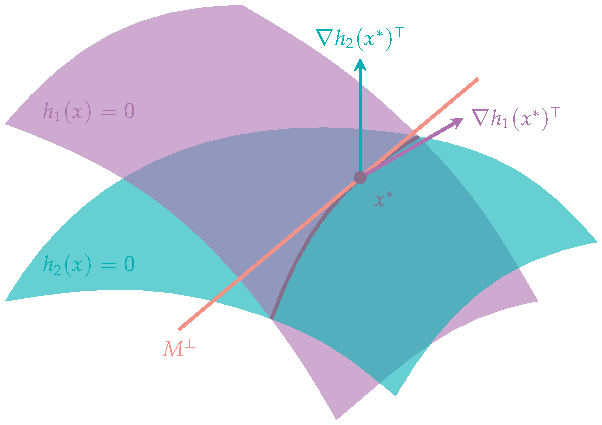
\includegraphics[width=0.8\textwidth]{figures/duality/tan-2constraint.pdf}
    \caption{正规点示意图}
    \label{fig:tan-2constraint}
\end{figure}

\begin{theorem}[正规点切空间刻画定理]\label{thm:tan-space-characterize}
设曲面$S\subseteq\R^n$由约束$h(x)=0$定义,$x^*\in S$是正规点,那么,
\[T_{x^*}(S)=M^\perp=\{{y:\nabla h(x^*)y=0}\}.\]
\end{theorem}
该定理的证明需要隐函数定理,对微积分要求较高,我们这里略去.

如此,针对正规点,我们找到了表达切空间的一种方法. 这一方法还揭示了曲面维度和约束的梯度向量的关系.

\begin{remark}
    实际上,梯度向量$\nabla h_i(x^*)$张成空间$M$的维数定义了曲面$S$在点$x^*$的维数. 如果在点$x^*\in S$一个邻域内维数都是$k$,那么,我们可以用一个$k$维的参数来描述这个邻域内的点. 这一性质被称为\textit{秩定理}.
\end{remark}

\section{条件极值与Lagrange乘子法}\label{sec:lagrange-multiplier}

有了切空间的准备,现在我们要对正规点推导带约束的优化问题的极值条件. 我们首先考虑只有等式约束的情况:

\begin{equation}
\begin{aligned}
\minimize_x\quad& f(x) \\
\text{s.t.}\quad& {h}(x)={0},\\
& x \in \Omega.
\end{aligned}    \label{eq:eq-constraint-only-differentiable}
\end{equation}
其中$f,h$都具有连续的一阶导数.

设$x^*$ 是一个约束$h(x)=0$一个正规点,同时也是函数$f$的一个在可行域中的极值点. 这一部分的目标是得到条件极值的一阶必要条件:
\begin{theorem}[条件极值的一阶必要条件]\label{thm:eq-opt-cond-1}
    令$x^*$是一个$f$的满足约束${h(x)=0}$的正规极值点. 那么存在一个${\lambda}\in \R^m$使得$$\nabla f(x^*)+{\lambda^\t \nabla h(x^*)=0}. $$
\end{theorem}

一阶必要条件$\nabla f(x^*)+{\lambda^\t}\nabla {h(x^*)=0}$以及约束${h(x^*)=0}$给出了$n+m$个等式以及包含${x^*,\lambda}$在内的$n+m$个变量. 因此在非退化的情况下,他们给出了一个唯一解. 

引入与这个约束问题对应的Lagrange函数:
        $$l({x,\lambda})=f(x)+{\lambda^\t h(x)}.$$
$\lambda$被称为\textit{Lagrange乘子}. 必要条件可以被写作:
\begin{align*}
    \nabla_x l({x,\lambda})&=0,\\
    \nabla_{\lambda} l({x,\lambda})&=0.
\end{align*}

这一个求解条件极值的方法会在大部分微积分课程中给出,我们这里的更重要的任务是给出这一方法的几何解释. 注意,\Cref{thm:eq-opt-cond-1} 本质上在说,$\nabla f(x^*)$是$\nabla h_i(x^*)$的线性组合,所以我们的目标就是得到这一事实. 

假设$h(x)=0$形成的曲面是$S$,考虑正规极值点$x^*\in S$. 我们任选一条曲线$x(t)$过$x^*=x(0.5)$,那么,$f(x(t))$在$t=0.5$处取得了极小值. 根据微积分的极值定理,我们有
\[\left.\frac{\d}{\d t}f(x(t))\right|_{t=0.5}=0\iff \nabla f(x^*)\dot{x}(0.5)=0.\]
因此,$\nabla f(x^*)$和切向量$\dot{x}(0.5)$正交,因为曲线$x(t)$是任意选取的,所以$\nabla f(x^*)$也和切空间$T_{x^*}(S)$正交.

现在,回忆\Cref{thm:tan-space-characterize},我们知道切空间$T_{x^*}(S)=M^\perp$,因此
\[\nabla f(x^*)^\t\in (M^\perp)^\perp=M=\left\{\sum_{i} \lambda_i \nabla h_i(x^*)^\t:\lambda_i\in\R\right\}.\]
换言之,$\nabla f(x^*)$是$\nabla h_i(x^*)$的线性组合,这就证明了\Cref{thm:eq-opt-cond-1}.


最后,作为应用,我们考虑一个例子.

\begin{example}[最大熵]\label{ex:max-entropy}
考虑一个离散的概率分布,其分布列为$p_i=\Pr(X=x_i),i=1,\dots,n$. 该分布的熵为
$$\epsilon = -\sum_{i=1}^n p_i \log p_i.$$
该分布的均值为$\sum_{i=1}^n x_i p_i$. 

如果均值固定为$m$,求解使熵最大化的参数可以被转化成以下问题:
\begin{align*}
\maximize_{p_i}\quad&-\sum_{i=1}^n p_i\log p_i \\
\text{s.t.}\quad& \sum_{i=1}^n p_i=1, \\
&\sum_{i=1}^n x_i p_i=m, \\
&p_i\geq 0, \qquad i=1,2,\dots,n.
\end{align*}

我们先忽略非负约束,假设这些约束不会被触发. 引入两个Lagrange乘子,$\lambda$和$\mu$,则Lagrange函数为
$$l=\sum_{i=1}^n (-p_i\log p_i+\lambda p_i+\mu x_ip_i)-\lambda-\mu m.$$
由一阶必要条件,$-\log p_i -1+\lambda+\mu x_i=0$,$i=1,2,\dots,n$. 因此,
$$p_i=\exp((\lambda-1)+\mu x_i),\quad i=1,2,\dots, n.$$
注意$p_i>0$,所以非负约束确实没有被触发. Lagrange乘子$\lambda$和$\mu$是两个用来保证等式约束被满足的参数. 
\end{example}

\section{Karush–Kuhn–Tucker条件}\label{sec:KKT}
现在加入不等式约束,考虑以下形式的问题:
\begin{equation}
\begin{aligned}
\minimize_x\quad& f(x) \\
\text{s.t.}\quad& h(x)=0, \\
&g(x)\leq 0,\\
& x \in \Omega.
\end{aligned}\label{eq:ineq-constraint-inequality-differentiable}
\end{equation}
其中$f,h,g$具有连续的一阶导数. 

我们将使用Lagrange乘子法来推导一阶必要条件. 现在,最主要的问题在于多了不等式约束,我们需要找到一种方法来处理这些约束.

假设$x^*$是一个极小值点,那么,我们可以将不等式约束$g(x)\leq 0$分为两部分:
\begin{itemize}
    \item $g_i(x^*)<0$. 根据$g_i$的连续性,在$x^*$的一个邻域内,恒有$g_i(x)<0$,因此这个约束在$x^*$附近一定不会违背. 我们称这样的约束为\textit{非激活约束}.
    \item $g_i(x^*)=0$. 如果稍微偏离$x^*$,那么$g_i(x)$可能会变成正数,因此,这个约束在$x^*$附近是起作用的. 我们称这样的约束为\textit{激活约束}.
\end{itemize}

因此,在$x^*$的一个邻域$U$内,如果激活的约束下标集是$J$,那么 \eqref{eq:ineq-constraint-inequality-differentiable} 可以被写作:
\begin{equation}
\begin{aligned}
    \minimize_x\quad& f(x) \\
    \text{s.t.}\quad& h(x)=0, \\
    &g_i(x)=0, \quad i\in J,\\
    & x \in U.
\end{aligned}
\label{eq:ineq-constraint-inequality-differentiable-active}
\end{equation}

根据这一观察,我们可以自然地推广正规点$x^*$的定义:
\begin{definition}[正规点]
考虑优化问题 \eqref{eq:ineq-constraint-inequality-differentiable},如果一个点$x^*$满足以下条件:
\begin{itemize}
    \item 它是可行域中的点:$h(x^*)=0$,$g(x^*)\leq 0$,$x\in\Omega$,
    \item 令$J$为满足$g_j(x^*)=0$的下标$j$的集合(激活的约束). 那么,梯度向量$\nabla h_i(x^*)$,$\nabla g_j(x^*)$,$1\leq i \leq m$,$j\in J$是线性无关的,
\end{itemize}
那么,$x^*$被称作该约束的\textbf{正规点}.
\end{definition}

换言之,此时的正规点不仅考虑等式约束,还要考虑起作用的(被激活的)不等式约束,这些不等式约束相当于等式约束. 类似Lagrange乘子法,此时的一阶必要条件为:

\begin{theorem}[Karush-Kuhn-Tucker条件]\label{thm:KKT}
令$x^*$为优化问题 \eqref{eq:ineq-constraint-inequality-differentiable} 的正规极小值点,那么,存在向量$\lambda\in\R^m$和向量$\mu\in \R^p$且$\mu\geq 0$使得
\begin{align}
    \nabla f(x^*)+\lambda^\t \nabla {h(x^*)}+\mu^\t \nabla g(x^*)&=0,\label{eq:KKT-1}\\
    {\mu^\t g(x^*)}&=0.\label{eq:KKT-2}
\end{align}
\end{theorem}

\begin{proof}
考虑$x^*$的邻域$U$,在这个邻域内,我们可以将问题 \eqref{eq:ineq-constraint-inequality-differentiable} 写作 \eqref{eq:ineq-constraint-inequality-differentiable-active},即只考虑激活的约束. 由于$x^*$是一个极小值点,根据\Cref{thm:eq-opt-cond-1},存在$\lambda\in\R^m,\mu\in\R^p$使得
\[
\nabla f(x^*)+\lambda^\t \nabla {h(x^*)}+\mu_J^\t \nabla g_J(x^*)=0.
\]
这里,$\nabla g_J(x^*)=(\nabla g_j(x^*))_{j\in J}$,即只考虑激活的约束.

对于非激活的下标$i$,我们补充定义$\mu_i=0$,于是,上式可以被写作
\[\nabla f(x^*)+\lambda^\t \nabla {h(x^*)}+\mu^\t \nabla g(x^*)=0.\]
这就得到了 \eqref{eq:KKT-1}.

对于被激活的下标$i$,我们有$g_i(x^*)=0$,因此,$\mu_i g_i(x^*)=0$;对于非激活的下标$i$,我们有$\mu_i=0$,因此,$\mu_i g_i(x^*)=0$. 于是,\eqref{eq:KKT-2} 得证.

最后,我们还需要证明$\mu\geq 0$. 因为$x^*$是\textit{可行域}内的极小值,所以,假设$x^*$沿着方向$y$使得恰好有一个$g_k$从激活变为非激活,因为此时还在可行域,$f$应该不变小. 

下面我们来选取这样的$y$. 考虑如下曲面:
\[S=\{x\in\R^n:h(x)=0,g_j(x)=0, j\in J\setminus\{k\}\}.\]
也就是除了$k$之外所有的等式约束形成的曲面. 我们从切空间$T_{x^*}(S)$中选取一个$y$,使得$\nabla g_k(x^*)y<0$,这样,$g_k$会从激活变为非激活,而其他约束依然得到满足. 这一选择的几何示意如\Cref{fig:select-y} 所示.

\begin{figure}[ht]
    \centering
    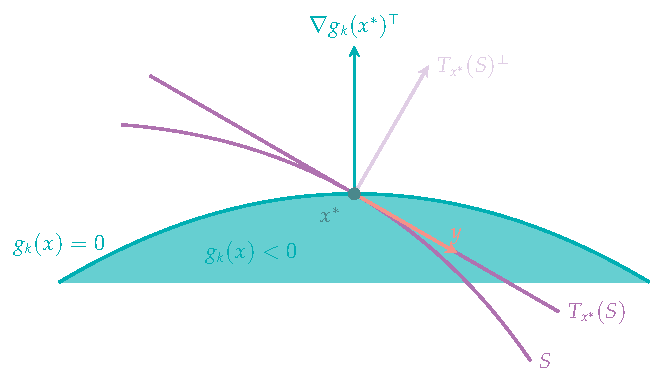
\includegraphics[width=0.8\textwidth]{figures/duality/select-y.pdf}
    \caption{选择$y$的几何示意}
    \label{fig:select-y}
\end{figure}

下面我们说明为什么这样的$y$存在. 因为$x^*$是正规点,所以根据\Cref{thm:tan-space-characterize},$T_{x^*}(S)=M^\perp$,其中

\[M=\left\{\sum_{i} \alpha_i \nabla h_i(x^*)^\t+\sum_{j\in J\setminus\{k\}} \beta_j \nabla g_j(x^*)^\t:\alpha_i,\beta_j\in\R\right\}.\]
根据正规点的定义,$\nabla g_k(x^*)^\t$不在$M$中,所以,$\nabla g_k(x^*)^\t$在$M^\perp$中的分量非零,于是,我们可以选择一个$y\in M^\perp$使得$\nabla g_k(x^*)y<0$. 

将$y$右乘 \eqref{eq:KKT-1},我们有
\[\nabla f(x^*)y+\lambda^\t \nabla h(x^*)y+\mu^\t \nabla g(x^*)y=0.\]
这等价于
\[\nabla f(x^*)y+\mu_k\nabla g_k(x^*)y=0.\]
令$x(t)$为一条在$S$内且经过$x^*$(此处$t=0$)的曲线,且有$\dot{x}(0)={y}$. 根据极小值的定义
\begin{align*}
    &0\leq \left.\frac{\d f(x(t))}{\d t}\right|_{t=0}=\nabla f(x^*)y=-\mu_k\underbrace{\nabla g_k(x^*)y}_{<0}.\\
    \iff&\mu_k\geq 0.
\end{align*}
这一证明对所有激活约束的$k$都成立,所以这就完成了证明. 
\end{proof}

条件 \eqref{eq:KKT-1} 对应的就是Lagrange乘子,而 \eqref{eq:KKT-2} 则是\textit{互补松弛条件}:

\begin{proposition}[互补松弛条件]
    对于一个优化问题 \eqref{eq:ineq-constraint-inequality-differentiable},考虑一个正规极小值点$x^*$和对应的Lagrange乘子$\lambda,\mu$. 我们有以下结论:
    \begin{itemize}
        \item $\mu\geq 0$;
        \item 如果$g_i(x^*)<0$,那么$\mu_i=0$;
        \item 如果$\mu_i>0$,那么$g_i(x^*)=0$.
    \end{itemize}
\end{proposition}

下面我们来看一个运用KKT条件的例子:
\begin{example}
考虑问题
\begin{align*}
    \minimize_{x_1,x_2} \quad &2x_1^2+2x_1x_2+x_2^2-10x_1-10x_2 \\
    \text{s.t.}\quad &x_1^2+x_2^2\leq 5, \\
    & 3x_1+x_2\leq 6.
\end{align*}
KKT条件为
\begin{align*}
    4x_1+2x_2-10+2\mu_1x_1+3\mu_2&=0, \\
    2x_1+2x_2-10+2\mu_1x_2+\mu_2&=0, \\
    \mu_1(x_1^2+x_2^2-5)&=0, \\
    \mu_2(3x_1+x_2-6)&=0,\\
    \mu_i&\geq 0,\quad i=1,2.
\end{align*}
为了求解此类问题,我们假设一些约束被激活,然后检查所得出的Lagrange乘子的符号正负. 在这个问题中,我们可以尝试假设有0,1,2个约束被激活. 

假设第一个约束被激活,第二个约束没有被激活,得出等式
\begin{align*}
4x_1+2x_2-10+2\mu_1x_1&=0, \\
2x_1+2x_2-10+2\mu_1x_2&=0, \\
x_1^2+x_2^2&=5.
\end{align*}
可得解$x_1=1,x_2=2,\mu_1=1.$

由于$3x_1+x_2=5$,因此第二个约束也被满足了. 因此,因为$\mu_1 > 0$,我们得出结论,这个解满足一阶必要条件. 
\end{example}

\section{Lagrange对偶}

\subsection{原始规划与对偶规划}

我们在推导KKT条件(\Cref{thm:KKT})的时候,最终得到了如下的Lagrange函数:
\[L(x,\lambda,\mu)=f(x)+\lambda^\t h(x)+\mu^\t g(x).\]
而KKT条件的第一条可以被写作
\[\nabla_x L(x,\lambda,\mu)=\nabla f(x)+\lambda^\t \nabla h(x)+\mu^\t \nabla g(x)=0.\]
换言之,这是给定$\lambda,\mu$之后$L$对$x$的一阶条件. 

现在,我们不再假设 \eqref{eq:ineq-constraint-inequality-differentiable} 中的 $f,h,g$ 具有一阶导数,只假定他们连续,此外,为简便起见,我们假设$\Omega=\R^n$,即不考虑集合约束. 我们的目标是求解
\begin{equation}
\begin{aligned}
    \minimize_x\quad& f(x) \\
    \text{s.t.}\quad& h(x)=0,\\
    & g(x)\leq 0, \\
    & x \in \R^n.
\end{aligned}\label{eq:non-differentiable-constraint}
\end{equation}

我们先说明,求解这一问题可以用Lagrange函数重写. 

\begin{proposition}\label{prop:lagrange-primal}
    优化问题 \eqref{eq:non-differentiable-constraint} 可以被写作
    \[\minimize_{x}\quad \sup_{\lambda,\mu\geq 0} L(x,\lambda,\mu).\]
    假设它的最优值为$p^*$,那么我们有:
    \begin{itemize}
        \item 当 \eqref{eq:non-differentiable-constraint} 无可行解时,$p^*=+\infty$;
        \item 当 \eqref{eq:non-differentiable-constraint} 有可行解时,$p^*$是 \eqref{eq:non-differentiable-constraint} 的最优值,对应的$x^*$是 \eqref{eq:non-differentiable-constraint} 的最优解.
    \end{itemize}
\end{proposition}
\begin{proof}
    我们只需要证明
    \[\sup_{\lambda,\mu\geq 0} L(x,\lambda,\mu)=\begin{cases}
        f(x),&\text{如果$x$满足约束},\\
        +\infty,&\text{其他情况}.
    \end{cases}\]

    当满足约束的时候,
    \[h(x)=0\implies \lambda^\t h(x)=0,\]
    \[g(x)\leq 0\implies \mu^\t g(x)\leq 0,\]
    因此,
    \[\sup_{\lambda,\mu\geq 0} L(x,\lambda,\mu)=L(x,\lambda,0)=f(x).\]

    当不满足约束的时候,我们有两种情况:
    \begin{itemize}
        \item 有某个$h_i(x)\neq 0$,所以可以取$\lambda_i$使得$\lambda_i h_i(x)$任意大,于是
        \[\sup_{\lambda,\mu\geq 0} L(x,\lambda,\mu)=+\infty.\]
        \item 有某个$g_i(x)>0$,所以可以取$\mu_i>0$使得$\mu_i g_i(x)$任意大,于是
        \[\sup_{\lambda,\mu\geq 0} L(x,\lambda,\mu)=+\infty.\]
    \end{itemize}
    这样,我们就完成了证明. 
\end{proof}

利用Lagrange函数,我们其实将一个有约束的问题变成了无约束的问题. 特别地,我们将优化问题转变为了\textit{原始规划}的形式:

\begin{definition}[原始规划和原始函数]
    优化问题 \eqref{eq:non-differentiable-constraint} 的\textbf{原始规划}是
    \[\minimize_{x}\quad \sup_{\lambda,\mu\geq 0} L(x,\lambda,\mu).\]
    其中,
    \[\omega(x)=\sup_{\lambda,\mu\geq 0} L(x,\lambda,\mu)\]
    被称为\textbf{原始函数}. 原始规划的最优值记为$p^*$.
\end{definition}

一个很自然的想法是,我们可以把$\min$和$\max$的顺序交换,这样我们就得到了\textit{对偶规划}.

\begin{definition}[对偶规划和对偶函数]
    优化问题 \eqref{eq:non-differentiable-constraint} 的\textbf{对偶规划}是
    \[\maximize_{\lambda,\mu\geq 0}\quad \inf_{x} L(x,\lambda,\mu).\]
    其中,
    \[\phi(\lambda,\mu)=\inf_{x} L(x,\lambda,\mu)\]
    被称为\textbf{对偶函数}. 对偶规划的最优值记为$d^*$.
\end{definition}

对偶函数并不是随手写出来的一个数学游戏,它有着很重要的意义. 我们回到本章开头的买家卖家小问题,对于乙(即买家),我们可以把最小化买入价这个问题抽象为

\begin{equation}
\begin{aligned}
    \minimize_y\quad& c^\t y \\
    \text{s.t.}\quad& Ay\geq b,\\
    & y\geq 0.
\end{aligned}\label{eq:linear-programming}
\end{equation}

它的Lagrange函数为
\[L(y,\mu)=c^\t y-\mu_1^\t (Ay-b)-\mu_2^\t y,\]
它的对偶函数为
\[\phi(\mu)=\inf_{y} L(y,\mu)=\inf_{y} c^\t y-\mu_1^\t (Ay-b)-\mu_2^\t y.\]
满足这一条件的$y$应该满足一阶条件:
\[\nabla_y L(y,\mu)=c-A^\t \mu_1-\mu_2=0,\]
只要确定了$\mu_1$就能确定$\mu_2$,所以可以将$\mu_2$消掉. 将上式的$\mu_2$代入$\phi(\mu)$,我们有
\begin{align*}
    \phi(\mu)&=\inf_{y} c^\t y-\mu_1^\t (Ay-b)-\mu_2^\t y\\
    &=c^\t y-\mu_1^\t (Ay-b)-\mu_2^\t y\\
    &=c^\t y-\mu_1^\t (Ay-b)-(c-A^\t \mu_1)^\t y\\
    &=\mu_1^\t b.
\end{align*}
此外,注意到$\mu_2\geq 0$,因此
\[
    0\leq \mu_2=c-A^\t \mu_1\implies A^\t \mu_1\leq c.
\]
因此,对偶规划为
\begin{equation}
\begin{aligned}
    \maximize_{\mu_1}\quad& b^\t \mu_1 \\
    \text{s.t.}\quad& A^\t \mu_1\leq c,\\
    & \mu_1\geq 0.
\end{aligned}\label{eq:linear-programming-dual}
\end{equation}
这正是我们在抽纸问题中甲的最大化自己纸浆售价的优化问题!

因此,我们可以想象,原始规划和对偶规划其实是买家和卖家的博弈,一个人希望最小化$L$,另一个人希望最大化$L$,这就是\textit{对偶性}的一个体现. 关于这一思路的详细讨论,请参阅\Cref{chap:game}. 

\begin{remark}
    以上过程实际上给出了一个通用的方法,求一个\textit{线性规划}的对偶规划. 
\end{remark}

\subsection{对偶的几何意义}

除了从博弈角度理解对偶,类似前面几节的讨论,我们也可以从几何角度理解对偶,这一理解将最后给我们带来\textit{弱对偶定理}和\textit{强对偶定理}.

考虑方程
\[L(x,\lambda,\mu)=b\iff f(x)+\lambda^\t h(x)+\mu^\t g(x)=b.\]
我们暂且省略$x$,于是,上面的式子可以被写作
\[\ell: f+\lambda^\t h+\mu^\t g=b.\]
如果我们固定$\lambda$和$\mu$,那么$\ell$定义了一个点$(f,h^\t,g^\t)^\t$形成的超平面,这个超平面的法向量是$(1,\lambda^\t,\mu^\t)^\t$. 反之,如果我们固定$(f,h,g)^\t$,那么$\ell$定义了一个点$(1,\lambda^\t,\mu^\t)^\t$形成的超平面,这个超平面的法向量是$(f,h^\t,g^\t)^\t$.

因此,对于$L$特定的取值,我们有一个点-超平面对应关系:我们可以把点重新看成超平面,超平面重新看成点. 这就是\textit{对偶性}的几何意义.

\begin{remark}
    实际上,这样的想法构成了\textit{射影几何}的核心. 在射影几何中,我们把无穷远处的点加入到几何空间中,然后研究这种几何的性质. 射影几何中,对偶性体现如下:任何命题,将点和线在命题中的位置互换,该命题仍然成立. 
\end{remark}

接下来,我们要阐述这一几何性质如何与优化问题联系起来. 定义集合
\[\mathcal{G}=\{(f(x),h(x)^\t,g(x)^\t)^\t:x\in\R^n\},\]
这是所有可能的$(f,h^\t,g^\t)^\t$形成的集合. 我们可以在一个坐标系中画出这个集合,如\Cref{fig:duality-G-set} 所示,为简化起见,我们总是忽略$h(x)$的影响.

\begin{figure}[htbp]
    \centering
    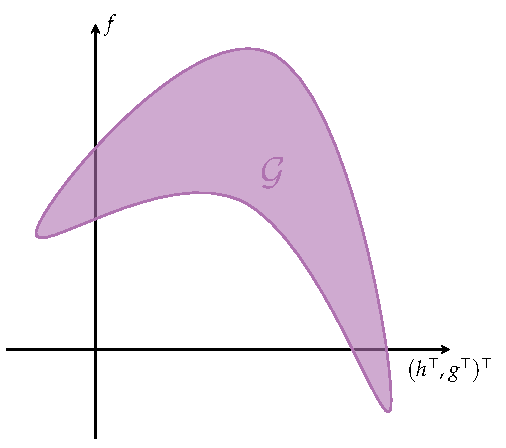
\includegraphics[width=0.7\textwidth]{figures/duality/duality-G-set.pdf}
    \caption{集合$\mathcal{G}$的示意图}
    \label{fig:duality-G-set}
\end{figure}

考虑$(t,u^\t,v^\t)^\t$形成的超平面
\[\alpha: t+\lambda^\t u+\mu^\t v= L(x,\lambda,\mu).\]
那么,这个超平面过点$(f(x),h(x)^\t,g(x)^\t)^\t$,并且法向量是$(1,\lambda^\t,\mu^\t)^\t$. 

令$u=v=0$,我们有$t=L(x,\lambda,\mu)$,这是$\alpha$在$t$轴上的截距. 因此,所有和$L$值相关的讨论都转变为了和$\alpha$的截距相关的讨论.

回忆原始函数的定义:
\[
\omega(x)=\sup_{\lambda,\mu\geq 0} L(x,\lambda,\mu)=\sup_{\lambda,\mu\geq 0} f(x)+\lambda^\t h(x)+\mu^\t g(x).
\]
因此,计算原始函数的过程其实就是,给定一个点$(t,u^\t,v^\t)^\t\in \mathcal{G}$,找到“斜率非负”的超平面,使得截距尽可能大. 

当$h(x)=0$且$g(x)\leq 0$的时候,这一截距一定在$\mu=0$的地方取到,因此,原始函数就是$\mathcal{G}$往$t$轴投影的值. 相应地,原始规划的最优值$p^*$就是$\mathcal{G}$左半区域的最低点的投影,如\Cref{fig:duality-primal-p-star} 所示.

\begin{figure}[htbp]
    \centering
    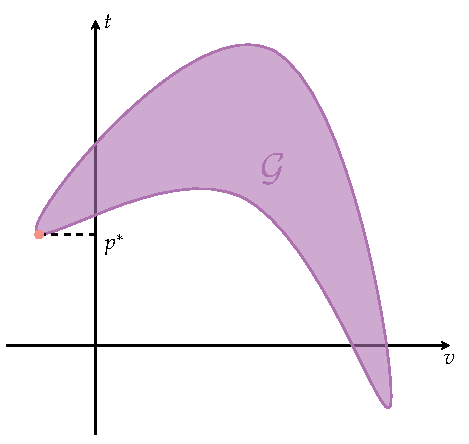
\includegraphics[width=0.7\textwidth]{figures/duality/duality-primal-p-star.pdf}
    \caption{原始规划的最优值$p^*$}
    \label{fig:duality-primal-p-star}
\end{figure}

根据最低点的性质,我们也可以把原始规划的最优值$p^*$看成是$\mathcal{G}$左半区域最低点切平面的截距.

那么,对偶规划是什么呢?回忆对偶函数的定义:
\[g(\lambda,\mu)=\inf_{x} L(x,\lambda,\mu)=\inf_{(t,u,v)\in\mathcal{G}} t+\lambda^\t u+\mu^\t v.\]
所以,这就是固定法向量$(1,\lambda^\t,\mu^\t)^\t$,找到过$\mathcal{G}$且截距最小的超平面,几何上看,这一超平面是在$\mathcal{G}$最低边缘的切平面(也就是只有切点而不会“穿过”$\mathcal{G}$). 相应地,对偶规划的最优值$d^*$就是这些切平面中最高的那个,如\Cref{fig:duality-dual-d-star} 所示.

\begin{figure}[htbp]
    \centering
    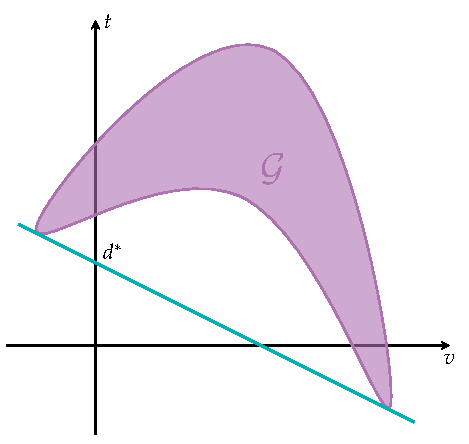
\includegraphics[width=0.7\textwidth]{figures/duality/duality-dual-d-star.pdf}
    \caption{对偶规划的最优值$d^*$}
    \label{fig:duality-dual-d-star}
\end{figure}

\subsection{弱对偶定理}

有了上述几何直观,我们可以阐述并证明\textit{弱对偶定理}.

\begin{theorem}[弱对偶定理]
    对于任意优化问题 \eqref{eq:non-differentiable-constraint},我们有
    \[d^*\leq p^*.\]
\end{theorem}

\begin{proof}
    直观上,$p^*$对应的是左半区域的最低点的切平面截距,它有可能会“穿过”$\mathcal{G}$的右半区域. 为了让这一现象不发生,我们可以把$p^*$对应的切平面进行旋转和下移,直到它只和$\mathcal{G}$下边缘切点接触. 这样,我们就得到了一个新的切平面,它的截距一定不会比$p^*$更大,因此,$d^*\leq p^*$. 这一过程见\Cref{fig:weak-duality}.

    \begin{figure}[ht]
        \centering
        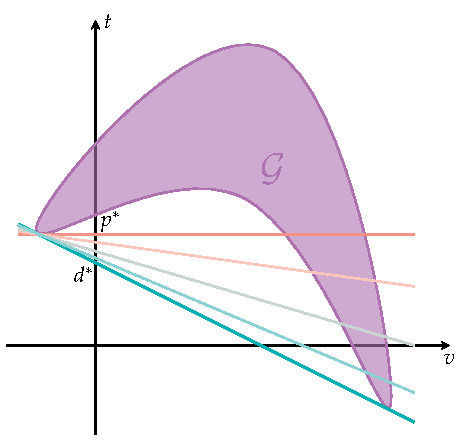
\includegraphics[width=0.7\textwidth]{figures/duality/weak-duality.pdf}
        \caption{弱对偶定理证明图示}
        \label{fig:weak-duality}    
    \end{figure}

    下面我们来严格叙述这一点. 对$\mu\geq 0$和$\lambda$,我们有
    \begin{align*}
        p^*&=\inf_{x} \sup_{\lambda,\mu\geq 0} L(x,\lambda,\mu)\\
           &\geq \inf_{x} L(x,\lambda,\mu)\\
           &=\phi(\lambda,\mu).       
    \end{align*}
    这里,第二个不等式就是在旋转切平面至法向量为$(1,\lambda^\t,\mu^\t)^\t$,然后使得它只和$\mathcal{G}$下边缘切点接触. 
    
    因此,$p^*\geq \phi(\lambda,\mu)$对所有$\lambda,\mu$都成立,于是也有$p^*\geq d^*$.
\end{proof}

\subsection{Slater条件,强对偶定理}

设原始规划对应的最低点为
    \[K=(f(x^*),h(x^*)^\t,g(x^*)^\t)^\t=(p^*,u^*,v^*)^\t,\]
从\Cref{fig:weak-duality} 看,如果$\mathcal G$完全位于过$K$的(水平)切平面上方并且$\mathcal G$在$t$轴左侧不为空,那么$p^*$和$d^*$一定是相等的,此时我们称之为\textit{强对偶定理}. 我们可以把这一条件形式化为\textit{凸规划}和\textit{Slater条件}.

\begin{definition}[凸规划]
    对于优化问题 \eqref{eq:non-differentiable-constraint},如果$f,g_i\,(i=1,\dots,p)$是凸函数,$h(x)$形如$Ax+b$,那么这个问题被称为\textbf{凸规划}. 这里,$A$是一个$m\times n$的矩阵,$b\in\R^m$.
\end{definition}

\begin{definition}[Slater条件]
    对于优化问题 \eqref{eq:non-differentiable-constraint},如果存在一个$x$使得$g(x)<0$且$h(x)=0$,那么这个问题满足\textbf{Slater条件}.
\end{definition}

容易看出,Slater条件意味着$\mathcal G$在$t$轴左侧不为空. 接下来,我们要说明,满足Slater条件的凸规划,$\mathcal G$完全位于过$K$的(水平)切平面上方. 为此,我们定义如下集合:
\[
\mathcal{G}^*=\{(t,u^\t,v^\t)^\t: \exists x\in\R^n, f(x)\leq t, h(x)=u, g(x)\leq v\}.
\]
如\Cref{fig:duality-G-star} 所示,$\mathcal{G}^*$是$\mathcal G$往右往上包络之后的集合. 

\begin{figure}[ht]
    \centering
    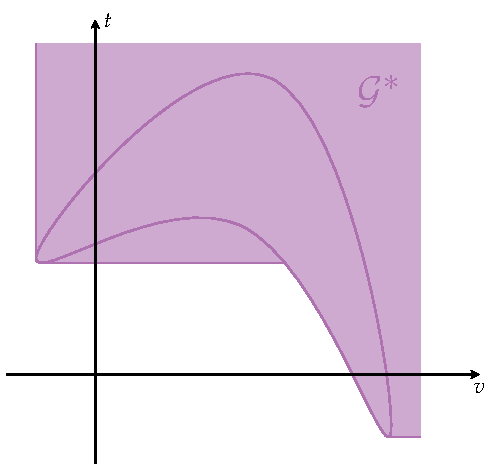
\includegraphics[width=0.7\textwidth]{figures/duality/duality-G-star.pdf}
    \caption{集合$\mathcal{G}^*$的示意图}
    \label{fig:duality-G-star}
\end{figure}

我们只要说明,包络之后的集合$\mathcal G^*$也完全位于该切平面上方,就能说明$\mathcal G$完全位于过$K$的该切平面上方. 下面,我们来证明这一点,从而证明强对偶定理.

首先我们证明$\mathcal G^*$是凸集.

\begin{lemma}\label{lemma:G*-convex}
    如果 \eqref{eq:non-differentiable-constraint} 是凸规划,那么$\mathcal G^*$是凸集.
\end{lemma}
\begin{proof}
    这一证明非常类似\Cref{thm:convex-epi} 的证明. 考虑$(t_1,u_1^\t,v_1^\t)^\t,(t_2,u_2^\t,v_2^\t)^\t\in\mathcal G^*$和$\theta\in[0,1]$,我们要证明
    \begin{equation}
        \theta(t_1,u_1^\t,v_1^\t)^\t+(1-\theta)(t_2,u_2^\t,v_2^\t)^\t\in\mathcal G^*.\label{eq:proof-G*-convex}
    \end{equation}
    
    根据定义,存在$x_1,x_2$使得
    \[f(x_1)\leq t_1, h(x_1)=u_1, g(x_1)\leq v_1,\]
    \[f(x_2)\leq t_2, h(x_2)=u_2, g(x_2)\leq v_2.\]
    令$x=\theta x_1+(1-\theta)x_2$,根据$f$和$g_i$的凸性,我们有
    \[f(x)\leq \theta f(x_1)+(1-\theta)f(x_2)\leq \theta t_1+(1-\theta)t_2,\]
    \[g_i(x)\leq \theta g_i(x_1)+(1-\theta)g_i(x_2)\leq \theta v_{1,i}+(1-\theta)v_{2,i}.\]
    根据$h$的定义,即$h(x)=Ax+b$,我们有
    \[h(x)=\theta h(x_1)+(1-\theta)h(x_2)=\theta u_1+(1-\theta)u_2.\]
    这样,我们就得到了 \eqref{eq:proof-G*-convex}. 因此,$\mathcal G^*$是凸集.
\end{proof}

接下来,我们说明$\mathcal G^*$完全位于过$K$的(水平)切平面上方,从而证明强对偶定理.

\begin{theorem}[强对偶定理]
    如果 \eqref{eq:non-differentiable-constraint} 是凸规划并且满足Slater条件,那么
    \[d^*=p^*.\]
    此外,如果$p^*$有限,那么存在$x^*\in\R^n$,$\lambda^*\in\R^m$和$\mu^*\in\R^p\,(\mu^*\geq 0)$使得
    \begin{equation}
        L(x^*,\lambda^*,\mu^*)=p^*=\sup_{\lambda,\mu\geq 0} L(x^*,\lambda,\mu)=\inf_{x} L(x,\lambda^*,\mu^*)=d^*.\label{eq:strong-duality-solution}
    \end{equation}
\end{theorem}
\begin{proof}
    如果$p^*=-\infty$,根据弱对偶定理,我们有$d^*\leq p^*=-\infty$,所以$d^*=-\infty=p^*$.

    注意,$p^*=+\infty$的情况是不可能的,因为Slater条件保证了至少有一个可行解. 
    
    现在假设$p^*$有限,此时,我们上面所描述的几何直观是有效的. 取$x^*$为原始规划的最优解,并记
    \[K=(f(x^*),h(x^*)^\t,g(x^*)^\t)^\t=(p^*,u^*,v^*)^\t.\]

    设$h(x)=Ax+b$,我们不妨设$A$是满秩矩阵,否则约束$h(x)=0$要么无法满足,要么有冗余的约束.

    根据\cref{lemma:G*-convex},$\mathcal G^*$是凸集. 我们需要选出来从$K$作出的切平面. 一个自然的选择是使用分离超平面定理(\Cref{thm:separation-hyperplane}). 定义另一个凸集为
    \[\mathcal{C}=\{(t,0,0)^\t: t<p^*\}.\]
    也就是一根恰好位于最低点下方的一个“杆”,见\Cref{fig:duality-proof-strong-dual}.

    \begin{figure}[ht]
        \centering
        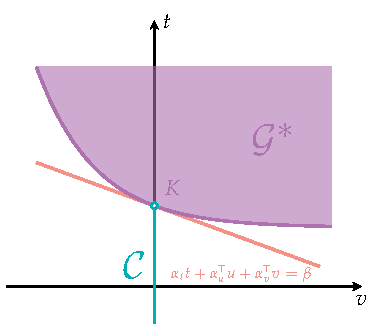
\includegraphics[width=0.6\textwidth]{figures/duality/duality-proof-strong-dual.pdf}
        \caption{分离超平面的图示}
        \label{fig:duality-proof-strong-dual}
    \end{figure}

    $K\in\mathcal G^*$,因而不为空,$\mathcal{C}$也不为空. 现在我们说明,$\mathcal G^*$和$\mathcal C$是不相交的. 假设$(t,u^\t,v^\t)^\t\in\mathcal G^*\cap \mathcal C$,那么存在$x$使得
    \[f(x)\leq t<p^*, h(x)=u=0, g(x)\leq v=0,\]
    这意味着$x$是一个可行解,但是它的目标值小于$p^*$,这与$p^*$的定义矛盾. 所以,没有这样的交点. 

    因此,我们可以用分离超平面定理(\Cref{thm:separation-hyperplane})找到一个非零$\alpha=(\alpha_t,\alpha_u^\t,\alpha_v^\t)^\t$和$\beta$使得
    \begin{align*}
        (t,u^\t,v^\t)^\t\in\mathcal G^*&\implies \alpha_t t+\alpha_u^\t u+\alpha_v^\t v\geq \beta,\\
        (t,0,0)^\t\in\mathcal C&\implies \alpha_t t\leq \beta.
    \end{align*}

    从几何上看,这一超平面就是过$K$作的切平面. 

    现在我们说明$\alpha_t\geq 0$并且$\alpha_v\geq 0$. 如不然,$\alpha_t<0$(或者$\alpha_v<0$)的话,我们可以取一个足够大的$t$(或者$v$)使得$\alpha_t t+\alpha_u^\t u+\alpha_v^\t v$任意小,这与第一个不等式矛盾.

    接下来,我们希望将这一分离超平面的系数与Lagrange函数对应起来,从而和前面对偶的几何意义联系起来. 换言之,我们希望取$\alpha_t=1$. 注意,$\alpha_t$是否为零决定了这一取法是否可行. 
    \begin{itemize}
        \item $\alpha_t>0$,此时,同时除以$\alpha_t$,即可不妨设$\alpha_t=1$. 根据$\mathcal G^*$的定义,
        \[(p^*,0,0)^\t\in\mathcal G^*\implies p^*\geq\beta.\]
        另一方面,第二个分离不等式直接得出
        \[p^*\leq\beta.\]
        因此,$p^*=\beta$. 所以$p^*$就是纵截距. 

        根据$\mathcal G^*$的定义,对任意$x$,
        \begin{align*}
            (f(x),h(x)^\t,g(x)^\t)^\t\in\mathcal G^*&\implies f(x)+\alpha_u^\t h(x)+\alpha_v^\t g(x)\geq p^*\\
            &\iff L(x,\alpha_u,\alpha_v)\geq p^*.
        \end{align*}
        因此,
        \[\varphi(\alpha_u,\alpha_v)=\inf_{x} L(x,\alpha_u,\alpha_v)\geq p^*.\]
        取$\lambda^*=\alpha_u$和$\mu^*=\alpha_v$,
        \[d^*=\sup_{\lambda,\mu\geq 0} \varphi(\lambda,\mu)\geq \varphi(\lambda^*,\mu^*)\geq p^*.\]
        根据弱对偶定理,$d^*\leq p^*$,所以$d^*=p^*$.

        考虑$x^*$,因为它是原始规划的最优解,所以
        \[p^*=\sup_{\lambda,\mu\geq 0} L(x^*,\lambda,\mu)\geq L(x^*,\lambda^*,\mu^*)\geq \inf_{x} L(x,\lambda^*,\mu^*)\geq p^*.\]
        结合$d^*=p^*$,我们就得到了 \eqref{eq:strong-duality-solution}.
        \item $\alpha_t=0$. 直观上,此时超平面平行于$t$轴,这意味着$\mathcal G$没有位于$t$轴左侧的点,也就是Slater条件不成立,这与我们的假设矛盾. 现在我们来严格说明这一点. 
        
        此时,对任意$x$,
        \[\alpha_u^\t h(x)+\alpha_v^\t g(x)\geq\beta\geq 0\cdot t=0,\]
        选择满足Slater条件的$\tilde{x}$,我们有
        \[\alpha_v^\t g_i(\tilde{x})\geq 0,\]
        因为对所有$i$,$g_i(\tilde{x})<0$,同时又有$\alpha_v\geq 0$,所以$\alpha_v=0$. 因为$\alpha\neq 0$,所以$\alpha_u\neq 0$. 于是,对任意$x\in\R^n$,
        \begin{equation}
            \alpha_u^\t h(x)=\alpha_u^\t(Ax+b)\geq 0. \label{eq:alpha_u-h}
        \end{equation}
        \[\alpha_u^\t (A\tilde{x}+b)=0,\]
        结合$A$是满秩矩阵,存在$x'\in\R^n$使得$\alpha_u^\t Ax'<0$,于是
        \[\alpha_u^\t (A(x'+\tilde{x})+b)<0,\]
        这与 \eqref{eq:alpha_u-h} 矛盾. 因此,这种情况实际上是不可能的.
    \end{itemize}
\end{proof}


\section{应用:支持向量机(SVM)}

作为前面极值必要条件的一个具体应用,我们考虑一个经典的机器学习分类器:\textit{支持向量机}(SVM). 

考虑二分类问题,输入$x\in \R^n$,函数$f$输出一个$\{-1,1\}$中的值. 二分类问题的学习问题指的是给定训练集$\{(x_i,y_i)\}_{i=1}^N$,找到$f$使得$f(x_i)=y_i$. 假设训练集是线性可分的,例如,存在某个$w\in \R^n$和$b\in \R$使得
    $$f(x)=\begin{cases}
		1,& w^\t x+b>0,\\
		-1, &w^\t x+b<0.
	\end{cases}$$

学习问题的首要目标是找到正确的以及最优的$w$和$b$. 本质上说,这就是一个\textit{找分离超平面}的过程. 那么,什么才叫最优呢?从几何视角来看,一个自然的想法是最大化\textit{分离距离},即训练集中所有点到分离超平面的距离和的最小值,见\Cref{fig:svm}.
\begin{figure}[ht]
    \centering
    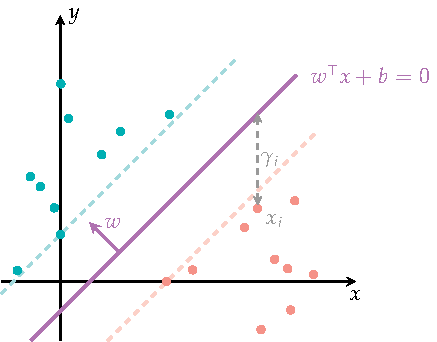
\includegraphics[width=0.65\textwidth]{figures/duality/svm.pdf}
    \caption{分离距离示意图.}
    \label{fig:svm}
\end{figure}

采样点$x_i$到分离超平面的归一化距离为
    $$\gamma_i=y_i\left(\left(\frac{w}{\norm{w}_2}\right)^\t x+\frac{b}{\norm{w}_2}\right).$$
$\gamma=\min_i\gamma_i$是最小的归一化距离. 于是我们的任务变成了最大化$\gamma$. 等价地,我们求解如下优化问题
\begin{align*}
    \maximize_{w,b}\quad&\gamma \\
    \text{s.t.}\quad&\gamma\le\gamma_i,\quad i=1,2,\dots,N.
\end{align*}

$\gamma\le\gamma_i$等价于$$y_i\left(\left(\frac{w}{\gamma\norm{w}_2}\right)^\t x+\frac{b}{\gamma\norm{w}_2}\right)\geq 1.$$
简洁起见,把$w$替换成$\frac{w}{\gamma\norm{w}_2}$,把$b$替换成$\frac{b}{\gamma\norm{w}_2}$,我们有$$y_i(w^\t x+b)\geq 1.$$
那么最大化$\gamma=\frac{1}{\norm{w}_2}$等价于最小化$\norm{w}_2^2$. 

我们得到以下凸规划问题:
\begin{align*}
    \min_{w,b}\quad&\frac{1}{2}\|w\|_2^2\\
    \text{s.t. }\quad &y_i(w^\t x_i+b)\geq 1,\quad i=1,2,\cdots, N.
\end{align*}

如何解决这个问题?利用上面的对偶理论,我们有如下步骤:
\begin{itemize}
    \item 写出Lagrange乘子和对偶规划(max-min).
    \item 验证Slater条件,于是只需要求解对偶规划.
    \item 利用KKT条件手动把对偶中的min消掉,得到一个二次规划.
    \item 用序列最小优化(SMO)等优化算法求解这个二次规划.
\end{itemize}

\section{习题}

\begin{enumerate}[wide, labelindent=0pt]
    \item 用Lagrange乘子法重新证明\Cref{prop:entropy-maximum}.
    \item \textbf{凸约束下的凸函数优化.} 考虑以下问题:
    \begin{enumerate}
        \item 已知在无约束条件下,满足一阶条件的局部最小值点也是一阶可微凸函数的全局最小值点,即$f'(x^*)=0\iff f(x)\ge f(x^*), \forall x\in \R^n$. 当引入凸集约束时,请举一个反例说明: 最小值点不一定满足一阶条件.
        \item 假设$f$是$\R^n$上的可微凸函数,$Q$是一个闭凸集. 证明:$x^*$是$f$在$Q$上的最小值点当且仅当对任意$x\in Q$,$\langle f'(x^*),x-x^*\rangle$.
    \end{enumerate}

    \item 判断并说明下列情况的可行点是否都是一阶正规点.
    \begin{enumerate}
    \item $n=3$, $m=2$, $x\in\R^3$, 等式约束$h_1(x) = x_1=0$, $h_2(x)=x_2-x_3^2=0$.
    \item $n=3$, $m=2$, $x\in \R^3$, 等式约束$h_1(x)=x_1-2x_2+1=0$, $h_2(x)=-x_1+x_2^2=0$.
    \end{enumerate}

    \item 考虑以下线性约束二次规划问题:
    \begin{align*}
    \min_x \quad&  \frac{1}{2}x^\t Qx\\
    \text{s.t.}\quad& Bx-b\le 0. 
    \end{align*}
    假设$Q$可逆.
    \begin{enumerate}
        \item 写出对偶规划,要求形如
        \begin{align*}
        \max_\mu \quad&  \varphi(\mu)\\
        \text{s.t.}\quad& \mu\geq 0. 
        \end{align*}
        \item 证明:对偶规划的一阶条件蕴含了原始规划的松弛互补条件.
    \end{enumerate}
    
    \item \textbf{双人零和博弈的Nash均衡}. 考虑一个双人零和博弈,玩家1可选择$n$种行动,玩家2可选择$m$种行动. 矩阵$A$中的元素$a_{ij}$表示玩家1选择行动$i$,玩家2选择行动$j$时,玩家1的收益$u_1(i,j)$. 对玩家2来说,他的收益$u_2(i,j)=-u_1(i,j)$. 玩家的混合策略是玩家行动的一个概率分布. 当玩家1和2分别采取行动$x$和$y$时,他们的期望收益分别是$x^\t Ay$和$-x^\t Ay$. 两个玩家的目标是最大化自己的期望收益.
    \begin{enumerate}
        \item 玩家1选取策略的方式是最大化自己的最小收益,即求$x^\star$达到$\max_x\min_y x^\t Ay$. 将该问题写为线性规划$P$.
        \item 玩家2选取策略的方式是最小化化对方的最大收益,即求$y^\star$达到$\min_y\max_x x^\t Ay$. 将该问题写为线性规划$P'$. 证明$P'$是$P$的对偶问题.
        \item 根据问题(2)的启发,证明minimax定理:
        \[\min_{x}\max_{y}x^\t Ay=\max_{y}\min_{x} x^\t Ay.\]
    \end{enumerate}
\end{enumerate}
